\documentclass[12pt,a4paper]{article}
\renewcommand{\thesection}{\Roman{section}}
\renewcommand{\thesubsection}{\thesection.\Roman{subsection}}
\usepackage{xeCJK}
\usepackage{caption}
\usepackage{amssymb}
\usepackage{amsmath}
\usepackage{geometry}
\usepackage{subfigure}
\usepackage{fancyhdr}
\usepackage[export]{adjustbox}
\usepackage{graphicx}
\graphicspath{{images/}}
\geometry{left=2.5cm,right=1.5cm,top=2cm,bottom=2cm}

\title{Deep Learning and Practice \\Lab3 \\ Report}
\date{April 18, 2019}
\author{呂紹篁, 0751904}
\setCJKmainfont{AR PL UKai CN}
\begin{document}
\captionsetup[figure]{labelfont={bf},labelformat={default},labelsep=period,name={Fig.}}
\thispagestyle{plain}
\cfoot{}
\maketitle

\section{Intoduction} \label{sec:intro}
In this lab, we will need to train models to classify diabetic retinopathy using PyTorch. To train our models, we have to write custom data loader to load our dataset. Then we will use ResNet \cite{he2016deep} architecture to train our model. To show the importance of pretrained coefficients in such huge network, with and without pretrained weights comparison is available. Finally, to evaluate the capabilities of our models, the confusion matrices are provided. 
\section{Experiment Setups} \label{sec:exp_setup}
\subsection{ResNet}
At first glance, we may think that the deeper the network, the stronger the model is. This statement may or may not be wrong. Fig.\ref{fig:resnet}(a) from \cite{he2016deep} illustrates training error and test error with 20-layer and 56-layer \textbf{plain} networks. Surprisingly, the deeper network has higher training error and higher test error. This is obvious not a overfitting problem since the training error still high. The problem comes from \textbf{degradation} of network: with the network depth increasing, accuarcy gets saturated and then degrades rapidly. 
He et al. proposed a deep residual learning framework which feedforward with shortcut connection an identity mapping to address the problem (Fig.\ref{fig:resnet}(b)). ResNet winned ILSVRC 2015 in image classification, detection and localization, as well as winned of MS COCO 2015 detection and segmentation. ResNet also gained best paper reward of CVPR in 2016. 

\begin{figure}[hbt]
\centering
\subfigure[Is Deeper Network Better?]{
  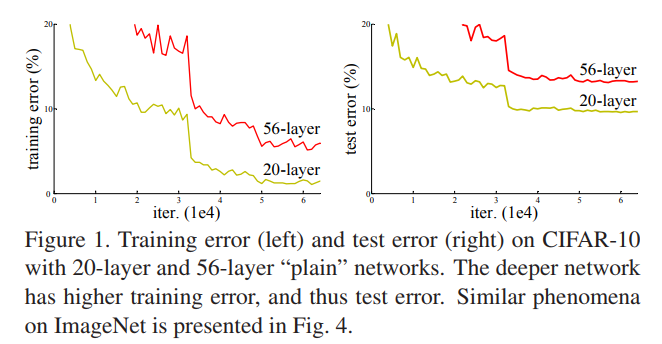
\includegraphics[scale=0.3]{deep.png}
}
\subfigure[Residual Learning]{
  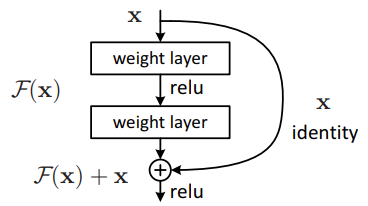
\includegraphics[scale=0.5]{res.png}
}
\caption{Residual Network}
\label{fig:resnet}
\end{figure}

\subsection{Dataloader}
To train our model, the story won't start without loading our dataset. PyTorch provides a convinent interface, \text{dataset}, for loading custom datasets from users. User only has to implement two methods, get the data and get the length of the dataset. After complete our dataset, we then throw it into the \text{dataloader} class with batch size (how many data we want to read one time). Our dataset is wrapped in \text{dataset.py} and converted to dataloader in Line 130 in \text{lab3.py}.

\subsection{Confusion Matrix}
Accuracy is a straightforward evaluation metric of a model. While if we have the prior knowledge that the probability of a disease will not occur is 0.99, our diagnostic test can always guess negative and gain high accuaracy, then accuracy is not a good metric at this time. Confusion matric is a common used metric to judge the capability of the model, it combined both ground truth and predicted result and divided data into 4 categories: \textbf{true positive} (TP), \textbf{true negative} (TN), \textbf{false positive} (FP) and \textbf{false negative} (FN). From example above, the meaning of 4 categories are shown in Table \ref{table:confuse}. Two metrics are derived from these four categories: \textbf{precision} and \textbf{recall} where $Precision=\frac{TP}{TP+FP}$ and $Recall=\frac{TP}{TP+FN}$, we can also get accuracy from $Accuracy=\frac{TP+TN}{TP+TN+FP+FN}$. Precision describes the ratio of correct predict in positive samples and recall describes the ratio of correct predict in samples which should be positive. So, if the disease has high infectivity, we may want the higher recall to prevent spread.

\begin{table}[hbt]
\begin{tabular}{|l|l|}
\hline
TP & The test shows the person has the disease and he indeed has              \\ \hline
TN & The test shows the person doesn't have the disease and he indeed doesn't \\ \hline
FP & The test shows the person has the disease while he doesn't               \\ \hline
FN & The test shows the person doesn't have the disease while he does have    \\ \hline
\end{tabular}
\caption{Simple Example of Confusion Matrix}
\label{table:confuse}
\end{table}

\section{Experimental Results} \label{sec:res}

\subsection{Highest Testing Accuracy}
The highest accuracy of each models are recorded in Table \ref{tab:highest}, where \textbf{No Pretrained} parts are trained in 10 epochs, for ResNet-18, we trained 40 epochs with batch size 60, and ResNet-50 20 epochs with size 15.
\begin{table}[hbt]
\centering
\begin{tabular}{|l|l|l|}
\hline
             & ResNet-18 & ResNet-50 \\ \hline
Pretrained   & \textbf{0.818}     & \textbf{0.822}     \\ \hline
NoPretrained & 0.735     & 0.733     \\ \hline
\end{tabular}
\caption{Highest Accuracy}
\label{tab:highest}
\end{table}

\subsection{Comparision} 
\begin{itemize} 
\item{Training and Testing Accuracy Curves} \\
Four model curves are illustrated in Fig. \ref{fig:result}.
\begin{figure}[hbt]
\centering
  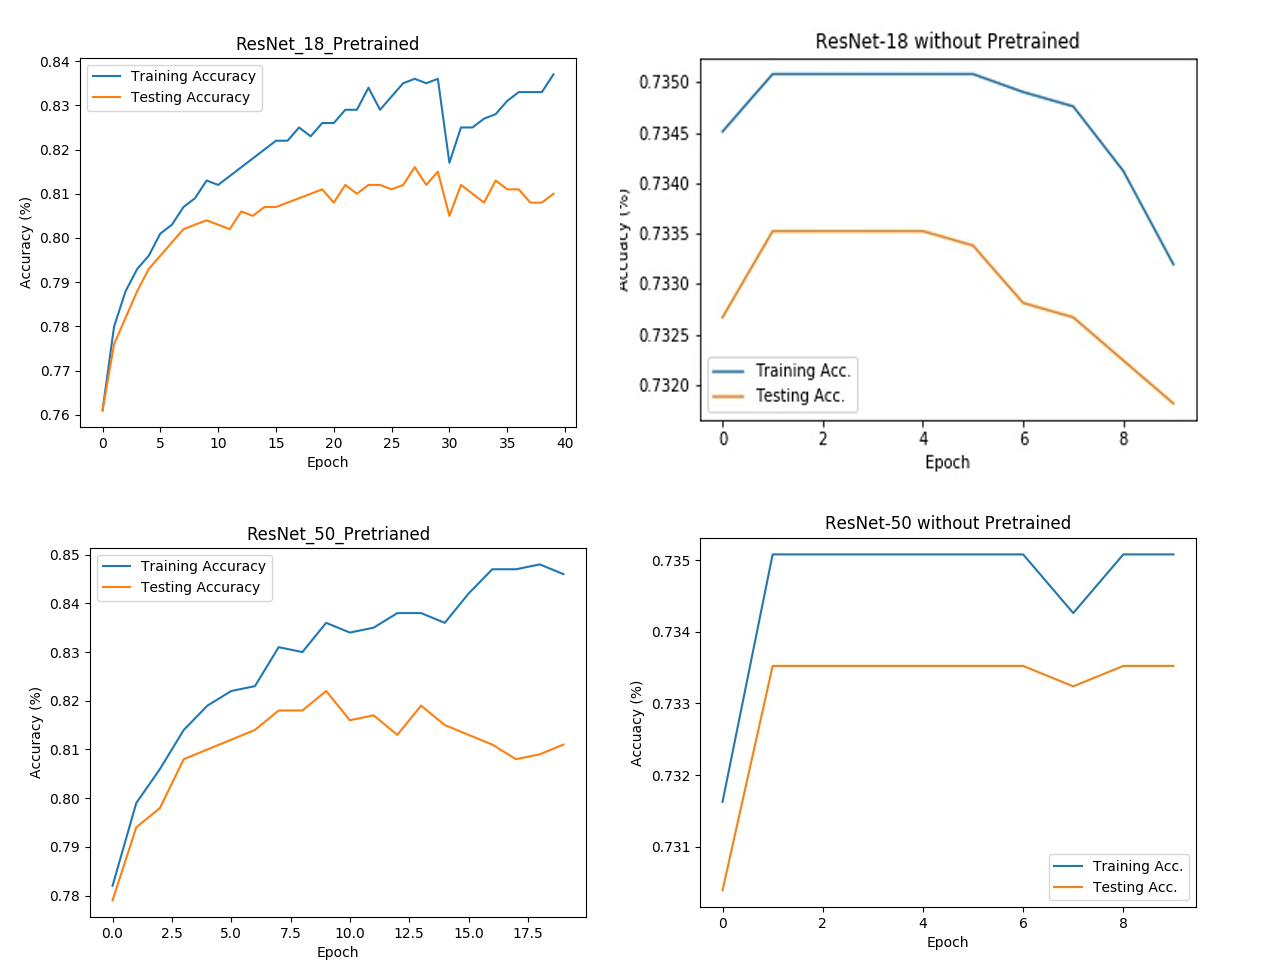
\includegraphics[scale=0.3]{result.png}
  \caption{Training and Testing Accuracy Curves. First row: ResNet-18, second row: ResNet-50, \\ left: with pretrained, right: without pretrained}
  \label{fig:result}
\end{figure}
\item{Confusion Matrix} \\
The confusion matrices of two with-pretrained models are shown in Fig. \ref{fig:con}. For a perfect model, the major diagonal of its confusion matrix should be \textbf{hot} (with higher value) since high correct prediction, while observes two figures below, they showed the similar patterns: it is hard to distinguish class 0, 1, 2 and class 2, 3, 4 (highly predict into class 0 and 2, respectively). We can also notice that the prediction of class 1 is extrmely tiny from the value of second column. While from the perspective of vision care, this model is acceptable because it can diagnose high-risk groups of eye diseases and does not have too high false positive for those low-risk groups. 
\begin{figure}[hbt]
\centering
  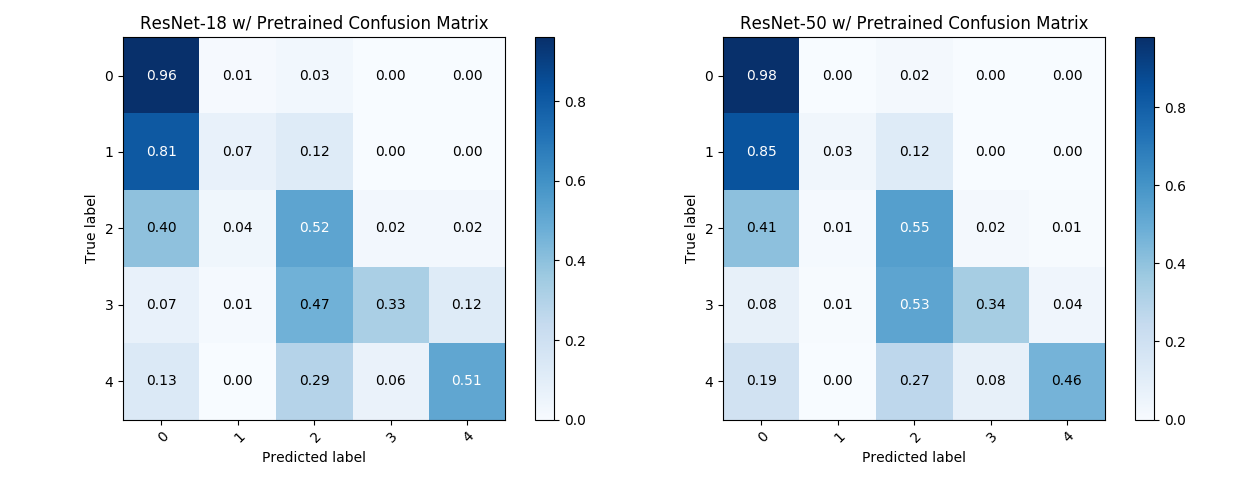
\includegraphics[scale=0.3]{confuse.png}
  \caption{Confusion Matrices of ResNet-18 and 50 With Pretrained}
  \label{fig:con}
\end{figure}
\end{itemize}


\section{Discussion} \label{sec:dis}
\begin{itemize}
\item{Time Consuming} \\
The lab this time is pretty time consuming. In my GeForce GTX 1070 machine, one epoch of training phase takes 7 minutes in ResNet-18 and 22 minutes in ResNet-50. If we want to gain accuracy higher than 82\%, we then have to train more epochs.
\item{Make Batch Size As Large As Possible} \\
After several trial, we notice that with larger batch size, we can get the better result. We used 60 for ResNet-18 and 15 for ResNet-50 which the usage of GPU memories is almost full load. Based on past experience, we test the model immediately after training phase, while if the memories is almost ran out, in test phase we will got cuda out of memories error, and we waste the time if we write to save the model after testing. So we divided the codes into two parts: one part keeps training with maximum batch size and saves the model after each epoch, the other tests the saved models and records the result accuracy.
\end{itemize}

\bibliographystyle{IEEEtran}
\bibliography{report.bib}

\end{document}
